\clearpage
\section{Processi di supporto}
\label{sec:proc_supp}
\subsection{Documentazione}
\label{sec:documentazione}
\subsubsection{Descrizione}
Verranno qui discusse le scelte intraprese per la scrittura, verifica ed approvazione della documentazione ufficiale di \emph{duckware}. Queste norme sono obbligatorie per tutti i documenti, i quali verranno elencati nella sottosezione \emph{Documenti correnti}.
\subsubsection{Ciclo di vita della documentazione}
Qualsiasi documento dovrà passare per gli stati di “\emph{Sviluppo}”, “\emph{Verifica}” ed “\emph{Approvato}”. Nel particolare, ciascuno di questi indica una fase precisa:
\begin{itemize}
    \item \textbf{Sviluppo}: Questa fase inizia con la creazione del documento e termina con la conclusione della stesura di tutte le sue parti. In questa fase i \emph{redattori} aggiungono le parti assegnate usando i \markg{ticket};
    \item \textbf{Verifica}: Questa fase inizia dopo l’assegnazione da parte del \emph{responsabile}. I \emph{verificatori} effettueranno i controlli necessari e, in caso di esito positivo, il documento entra automaticamente nella fase “\emph{Approvato}”. In caso di esito negativo sarà necessario che il \emph{responsabile} di progetto riassegni il documento ad un \emph{redattore} attraverso una nuova fase di "\emph{Sviluppo}";
    \item \textbf{Approvato}: Questa fase coincide con il completamento della parte di "\emph{Verifica}" avvenuta con successo nella quale il verificatore certifica la correttezza. Il documento verrà dunque consegnato al \emph{responsabile} il quale lo approverà per il rilascio esterno.
\end{itemize}

\subsubsection{Separazione tra documenti interni ed esterni}
Ogni documento dovrà avere una specifica classificazione. Vi saranno sia documenti \textbf{interni} in lingua italiana che verranno utilizzati da \emph{duckware} internamente, sia documenti \textbf{esterni} che verranno condivisi con \emph{la Proponente} ed i committenti. Questi ultimi potrebbero essere scritti in lingua inglese nel caso potesse essere utile al fine di soddisfare le richieste di deploy dell’utente finale.

\subsubsection{Nomenclatura dei documenti}
Ogni documento, tranne la Lettera di Presentazione ed i Verbali, adotteranno questo schema di nomenclatura:
\begin{itemize}
    \item \textbf{NomeDocumento}: indica il nome del documento e dovrà essere senza spazi con il vincolo di avere una lettera maiuscola all’inizio di ogni parola;
    \item \textbf{vX.Y.Z}: indica il numero versionamento.
\end{itemize}
Nel particolare, il versionamento sarà composto da tre numeri interi, separati da un punto, con il seguente significato:
\begin{itemize}
    \item \textbf{X}: rappresenta il numero di pubblicazioni ufficiali del documento e ad ogni suo incremento corrisponde un azzeramento di Y e Z;
    \item \textbf{Y}: rappresenta il numero di verifiche terminate con successo e ad ogni suo incremento corrisponde un azzeramento di Z;
    \item \textbf{Z}: rappresenta il numero di modifiche effettuate al documento durante lo sviluppo.
\end{itemize}
Ogni documento sarà redatto all’interno di un file .tex e solamente dopo lo stato di “Approvato” verrà generato il relativo PDF che conterrà la versione definitiva approvata dal \emph{responsabile} di progetto.

\subsubsection{Documenti correnti}
Verranno ora esposti i documenti formali, in ordine alfabetico, e divisi per appartenenza (Interno ed Esterno):\\[0.5cm]
\textbf{ESTERNO}
\begin{itemize}
    \item \textbf{[ AdR ] - Analisi dei Requisiti}: Questo documento viene redatto agli \emph{Analisti} dopo che questi ultimi hanno analizzato il capitolato e interagito con il proponente. All’interno dell’analisi dei requisiti saranno esposti tutti i requisiti del progetto, inclusi i diagrammi di interazione con l’utente ed i casi d’uso;
    \item \textbf{[ GL ] - Glossario}: Documento che raccoglie tutti i termini che verranno usati nei documenti formali; serve a disambiguare termini o a facilitarne la comprensione;
    \item \textbf{[ PdP ] - Piano di progetto}: Documento che tratta della pianificazione e dell’analisi della gestione delle risorse di tempo;
    \item \textbf{[ PdQ ] - Piano di qualifica}: Tale documento descrive gli obiettivi che il gruppo sarà tenuto a soddisfare al fine di garantire la qualità del prodotto e del processo.
\end{itemize}
\textbf{INTERNO}
\begin{itemize}
    \item \textbf{[ NdP ] - Norme di progetto}: Documento che descrive gli standard adottati da \emph{duckware} durante lo sviluppo del progetto scelto;
    \item \textbf{[ SdF ] - Studio di fattibilità}: Documento che analizza i pregi ed i punti a sfavore di ogni capitolato con le relative riflessioni che hanno portato \emph{duckware} alla sua scelta finale.

\end{itemize}

\subsubsection{Norme}
\paragraph{Struttura dei documenti}\mbox{}\\[0.4cm]
Ogni documento presentato è stato realizzato seguendo uno schema generale che dovrà essere rispettato in ogni documento ufficiale, fatta eccezione della lettera di presentazione e dei verbali. I criteri sono i seguenti:
\begin{itemize}
    \item \textbf{Frontespizio}: sezione presente nella prima pagina di ogni documento e conterrà il logo di \emph{duckware}, il titolo del relativo documento, la versione del documenti, il nome del gruppo ed il nome del progetto;
    \item \textbf{Informazioni sul documento}: si compone di una lista di responsabili, verificatori, redattori del documento e della tipologia d’uso del documento, una breve descrizione del contenuto e, a fondo pagina, numero di versione corrente e data di quando è stato modificato per l'ultima volta il documento;
    \item \textbf{Diario delle modifiche}: sarà presente nella seconda pagina di ogni documento e conterrà una tabella, ordinata in modo decrescente per data, delle modifiche apportate al documento. Nello specifico, ogni riga conterrà: versione, data, descrizione delle modifiche, autore e ruolo;
    \item \textbf{Indice delle sezioni}: si tratta di un elenco degli argomenti trattati nel documento che conterrà: titolo, argomento e numero pagina;
    \item \textbf{Indice delle tabelle}: sezione che contiene l’elenco delle tabelle e ha la stessa struttura dell’indice delle sezioni;
    \item \textbf{Introduzione}: contiene lo scopo del documento, le informazioni sul glossario ed i riferimenti utili normativi ed informativi;
    \item \textbf{Contenuto del documento}: tutto ciò che non è stato elencato nei precedenti punti, verrà trattato all’interno del documento.
\end{itemize}
\paragraph{Norme tipografiche}\mbox{}\\[0.4cm]
\begin{itemize}
    \item \textbf{Intestazione}: in ogni pagina del documento dopo il frontespizio ci sarà sulla sinistra il nome del capitolo corrente e sulla destra il logo di \emph{duckware};
    \item \textbf{Parentesi}: le parentesi tonde descrivono esempi e forniscono sinonimi, le quadre rappresentano uno standard ISO o un riferimento ad un codice definito all’interno del documento stesso;
    \item \textbf{Piè di pagina}: a sinistra c’è il nome del documento, a destra il numero di pagina;
    \item \textbf{Stile del testo}
    \begin{itemize}
        \item Corsivo: dà enfasi ad un termine o concetto;
        \item Grassetto: per i titoli, sottotitoli o termini all’interno di elenchi o liste.
    \end{itemize}
    \item \textbf{Formati}
    \begin{itemize}
        \item \emph{Date}: ogni data verrà formattata secondo il formato dd-mm-yyyy dove dd indica il giorno (a una o due cifre), mm il mese (a due cifre o in forma letterale estesa) e yyyy l’anno (sempre a quattro cifre). Solo il \emph{Registro delle Modifiche} fa eccezione a questa regola, in quanto la data   adotterà il formato yyyy-mm-dd, per dare risalto all'andamento cronologico delle iterazioni sul documento;
        \item \emph{Grassetto}: va utilizzato per i titoli di paragrafi e per i titoli di elementi in elenco;
        \item \emph{URI}: ogni URI sarà in corsivo e di colore blue di modo da essere conformi agli standard degli URI nelle pagine web.
    \end{itemize}
    \item \textbf{Riferimenti informativi}: Ogni riferimento esterno al progetto, come ad esempio guide o software, dovrà essere indicato a piè di pagina;
    \item \textbf{Nomi}: sono stati realizzati comandi personalizzati per richiamare la visualizzazione dei seguenti termini:
    \begin{itemize}
        \item \texttt{\textbackslash groupName} visualizza il nome del gruppo, "duckware";
        \item \texttt{\textbackslash groupEmail} visualizza l'indirizzo email del gruppo, "duckware.swe@gmail.com";
        \item \texttt{\textbackslash verif} è un comando che, tramite l'utilizzo di \texttt{\textbackslash renewcommand} posto all'inizio del file .tex principale, permette di visualizzare i nomi dei verificatori assegnati al documento;
        \item \texttt{\textbackslash resp} come il comando precedente, visualizza il nome del responsabile del documento;
        \item \texttt{\textbackslash editorfrow} e \texttt{\textbackslash editorsrow} inseriscono nel documento i nomi dei redattori del documento, rispettivamente nella prima e nella seconda riga;
        \item Sono stati creati dei comandi specifici per i nomi dei singoli componenti dei gruppi, in modo da semplificare e velocizzare la creazione dei documenti. Esempio: \texttt{\textbackslash luca} visualizzerà il nome nel formato "Luca \textsc{Stocco}";
        \item Per standardizzare la nomenclatura dei documenti, sono stati aggiunti dei comandi appositi. Esempio: \texttt{\textbackslash pdp} visualizzerà il nome del documento nel formato "Piano di Progetto".
    \end{itemize}
    \item \textbf{Componenti grafiche}: sono ammessi formati PNG e JPG ma sono preferibili immagini informato SVG poiche queste ultime preservano una maggiore qualità anche in caso di ridimensionamento.
\end{itemize}
È stato creato un template di documentazione che potrà essere impiegato per la realizzazione dei vari documenti ufficiali. Questo template è conforme a tutte le norme di documentazione esposte nelle precedenti sezioni.
\subsubsection{Ambiente}
La scrittura dei documenti dovrà essere realizzata con \markg{TexStudio} o \markg{TexMaker}, due ambienti di scrittura integrato per la creazione di documenti LaTeX. Questi software rendono la scrittura LaTeX semplice e confortevole oltre che fornire numerose funzionalità come l'evidenziazione della sintassi, il visualizzatore integrato, il controllo dei riferimenti e vari assistenti.\\Per maggiori dettagli:
\begin{itemize}
    \item TeXstudio\footnote{\href{https://www.texstudio.org/}{https://www.texstudio.org/}};
    \item TexMaker\footnote{\href{http://www.xm1math.net/texmaker/}{http://www.xm1math.net/texmaker/}};
\end{itemize}
\subsubsection{Strumenti di supporto}
Per facilitare e velocizzare la manutenzione della documentazione è stato realizzato un programma per automatizzare l’esecuzione di certe attività. Sarà possibile utilizzare questo programma in qualsiasi sistema operativo che abbia .NET Framework installato. Il programma \texttt{GlossaryHelper.exe} facilita la manutenzione e l’aggiornamento del glossario e di tutti i suoi documenti, nel particolare, si tratta di un eseguibile dotato di GUI in grado di:
\begin{itemize}
    \item Caricare il file *.tex relativo al glossario per inserire e/o rimuovere termini al suo interno. Il programma verificherà la presenza di duplicati nei termini del glossario e, in caso ce ne siano, impedirà l’inserimento;
    \item In seguito all’aggiunta o alla rimozione di termini dal glossario, sarà possibile aggiornare tutti i file dei documenti. Sarà sufficiente specificare al programma la cartella root contenente i documenti da analizzare ed il programma avrà cura di selezionare ogni file *.tex per procedere all’aggiornamento.
\end{itemize}
Per poter eseguire il programma è consigliabile avere installata l’ultima versione di .NET Framework, tuttavia il requisito minimo è quello di avere il supporto per .NET Framework 4.7.2 (per C\# 7.1).
\subsection{Qualità}
\label{sec:qualita}
\subsubsection{Descrizione}
Questa sezione descrive le procedure per il calcolo dei parametri descritti nel Piano di qualifica.
\subsubsection{Classificazione dei processi}
Per garantire la qualità del lavoro, gli Amministratori hanno suddiviso il lavoro in vari processi che sono stati poi riportati nel \emph{Piano di Qualifica}. Dovrà essere rispettata la notazione \textbf{PROC[value]}  dove \textbf{value} indica il codice univoco del processo tramite un numero intero a tre cifre che parte da 1 ed incrementa per ogni unità.
\subsubsection{Classificazione delle metriche}
Per garantire la qualità del lavoro fatto gli Amministratori hanno definito delle metriche che rispettano la seguente notazione \textbf{M[categ][macro categ][num]} oppure \textbf{M[categ][macro categ][num][sottonum]}dove:
\begin{itemize}
    \item \textbf{categ}: va ad indicare la categoria della metrica ed assume i seguenti valori:
    \begin{itemize}
        \item \textbf{PRC}: per indicare i processi;
        \item \textbf{PRD}: per indicare i prodotti;
        \item \textbf{PDT}: per indicare i test.
    \end{itemize} 
\end{itemize}
\begin{itemize}
    \item \textbf{macrocateg}: indica la macrocategoria della metrica, se esiste altrimenti non compare.\\
    Per le metriche di prodotto \textbf{PRD} può assumere i valori:
    \begin{itemize}
        \item \textbf{D}: per indicare i documenti;
        \item \textbf{S}: per indicare il software.
    \end{itemize}
\end{itemize}
\begin{itemize}
    \item \textbf{num}: va ad indicare il codice univoco della metrica come numero intero a tre cifre a partire da 1. Esempio \textbf{MPRC001}.
    \item \textbf{sottonum}: va ad indicare il codice univoco di una sotto-metrica appartenente alla metrica padre, con un numero intero ad una cifra a partire da 1. Esempio \textbf{MPRC001.1} è una sotto-metrica della metrica \textbf{MPRC001}.
\end{itemize}

\subsubsection{Controllo di qualità di processo}
La qualità dei processi verrà garantita dal metodo \markg{PDCA}, descritto nell'appendice A. Grazie a tale metodo si potrà ottenere un miglioramento continuo della qualità di tutti i processi, inclusa la verifica. Per ottenere la qualità dei processi bisogna:
\begin{itemize}
    \item Definire il processo affinchè esso sia controllabile;
    \item Controllare il processo in funzione del raggiungimento di un alto livello di efficacia ed efficienza;
    \item Usare strumenti di valutazione quali PDCA e \markg{SPICE}.
\end{itemize}
\subsection{Configurazione}
\label{sec:configurazione}
\subsubsection{Controllo di versione}
\paragraph{Descrizione}\mbox{}\\[0.4cm]
Per le parti versionabili del progetto e per i documenti ufficiali si è scelto l’utilizzo di GitLab, la condivisione per documenti informali ed altro materiale di supporto durante lo sviluppo del progetto avviene per mezzo di \markg{Google Drive}.
\paragraph{Struttura della repository}%TODO mi da errore da qui: \\[0.4cm]
Nella root della \markg{repository} sono presenti 4 cartelle: 
\begin{itemize}
    \item \textbf{firme:} contiene le immagini delle firme dei componenti del gruppo;
    \item \textbf{Template\_{}latex:} contiene i file \texttt{.tex} che gestiscono i comandi personalizzati, i comandi di formattazione delle pagine, i packages da includere per poter compilare con successo i documenti, il logo, le definizioni del glossario, le entries per stilare la bibliografia (se necessaria o richiesta). Inoltre contiene a sua volta le cartelle \emph{esempio\_{}documento} e \emph{esempio\_{}verbale} che descrivono come devono essere strutturate le cartelle dei singoli documenti;
    \item \textbf{Tools:} in questa cartella verranno inseriti tutti gli strumenti di utilità, come ad esempio \texttt{GlossaryHelper.exe};
    \item \textbf{RR:} questa cartella contiene tutti i documenti relativi alla \textit{Revisione dei Requisiti}.
    \item \textbf{RP:} questa cartella contiene tutti i documenti relativi alla \textit{Revisione di Progettazione}.
\end{itemize}
Nella cartella \textbf{RR} vengono distinti i documenti a seconda del loro utilizzo:
\begin{itemize}
    \item Nella \textbf{Cartella Esterni} sono presenti altre sotto cartelle con all'interno i documenti correlati:
    \begin{itemize}
        \item Analisi dei requisiti;
        \item Glossario;
        \item Piano di progetto;
        \item Piano di qualifica;
        \item Verbali.
    \end{itemize}
    \item Nella \textbf{Cartella Interni} invece troviamo le apposite cartelle per i seguenti documenti:
    \begin{itemize}
        \item Glossario;
        \item Studio di fattibilità; 
        \item Norme di progetto;
        \item Verbali interni.
    \end{itemize}
\end{itemize}
La cartella \textbf{RP} avrà la stessa struttura della cartella \textbf{RR}. Verranno create successivamente altre directory in base alle necessità che si presenteranno durante lo sviluppo del progetto, come ad esempio la cartella \emph{includes} presente in ogni sotto cartella dei documenti e che racchiude tutti i file inclusi solo in quello specifico documento. All’interno di ogni cartella vi è un file LaTeX che assume il nome del documento e la sua versione attuale.
\paragraph{Ciclo di vita dei branch}\mbox{}\\[0.4cm]
Per migliorare l'efficienza e l'efficacia di sviluppo, sono stati creati dei branch, denominati con il nome del rispettivo documento in redazione.
Inoltre, è presente un branch di lavoro, chiamato \texttt{develop} nel quale confluiranno tutti i branch, una volta approvati i singoli documenti.
Una volta che tutti i documenti sono stati {verificati ed approvati, si raggiunge una fase chiamata \markg{milestone}, e si può dunque procedere ad effettuare una \markg{release}. 
I documenti della saranno contenuti nel branch \texttt{master}.
\paragraph{Aggiornamento della repository}\mbox{}\\[0.4cm]
Per l’aggiornamento della repository verranno usati i seguenti comandi Git:
\begin{itemize}
    \item "git status": per verificare in che branch ci si trova. Inoltre questo    comando permette di tenere sotto controllo le modifiche locali fatte ai file;
    \item "git checkout \emph{nomeBranch}": permette di spostarsi nel branch indicato;
    \item "git pull": permette di aggiornare la repository locale;
    \item "git add \emph{nomeFile}": aggiunge il file specificato all'\markg{area di staging};
    \item "git add .": aggiunge tutti i file che sono stati modificati all'area di staging;
    \item "git commit": permette di salvare le modifiche aggiunte in area di staging al repository locale;
    \item "git push": sincronizza il repository remoto con quello locale.
\end{itemize}
\subsubsection{Strumenti}
\begin{itemize}
    \item Server git: è stato utilizzato GitLab per l’affidabilità e il supporto a continuous integration;
    \item Client git: sono state utilizzate le applicazioni GitKraken (per sistemi operativi basati su Linux) e GitHub Desktop (per sistemi MacOS e Windows), oltre agli strumenti da linea di comando.
\end{itemize}
\subsection{Procedure di controllo di qualità di processo}
\label{sec:controllo_qualita}
Per assicurare la qualità del prodotto finale è necessario perseguire la qualità dei processi che lo definiscono. Per adempiere a tale obbiettivo è stato deciso di seguire un'organizzazione interna dei processi incentrata sul principio del miglioramento continuo: PDCA (Plan, Do, Check, Act) e di adottare lo standard ISO/IEC 15504, conosciuto come SPICE (Software Process Improvement and Capability Deter- mination), contenente un modello di riferimento che definisce una dimensione del processo ed una dimensione della capacità.
Per ottenere qualità sui processi è necessario:
\begin{itemize}
    \item \textbf{Definire il processo}\\ In modo tale che sia controllabile
    \item \textbf{Controllare il processo}\\ Con l'obbiettivo di ottenere efficacia ed efficienza  
    \item \textbf{Usare strumenti di valutazione}\\ PDCA e SPICE
\end{itemize}
\subsection{Metriche qualità per il processo}
\label{sec:qualita_processo}
Verranno utilizzate le seguenti metriche per valutare l’efficienza e l’efficacia dei processi. Saranno quindi fatte delle misurazioni periodiche delle metriche, circa ogni 7 giorni da inizio a fine revisione, sui processi per quantificare l'andamento della qualità
\subsubsection{MPRC001 - Schedule Variance}
Si tratta di una formala che indica se una pianificazione del progetto è in linea con la schedulazione temporale delle attività. Essa si calcola attraverso la seguente formula:
\begin{displaymath}
    SV = BCWP - BCWS
\end{displaymath}
\begin{itemize}
    \item \textbf{BCWP}: valore delle attività completate al momento del calcolo;
    \item \textbf{BCWS}: valore pianificato per realizzare le attività.
\end{itemize}
Il risultato ne segue un valore positivo, indice di una velocizzazione nello svolgimento dei processi, o un valore negativo, indice di un rallentamento.
\subsubsection{MPRC002 - Budget Variance}
Questa formula mostra se i costi sono stati previsti correttamente attraverso la seguente formula:
\begin{displaymath}
    BV = BCWS - ACWP
\end{displaymath}
\begin{itemize}
    \item \textbf{BCWS}: costo sostenuto fino al momento del calcolo;
    \item \textbf{ACWP}: valore pianificato per la realizzazione delle attività.
\end{itemize}
Il risultato ne segue un valore positivo, indice di una spesa più bassa rispetto a quanto pianificato in precedenza, o un valore negativo, indice di una spesa fuori dal budget.

\subsubsection{MPRC003 - Rischi non previsti}
Valore numerico che indica la quantità di rischi esterni presenti ed elencati nel documento Analisi dei Rischi v2.0.0 riscontrati nella corrente fase di progetto. Si tratta di un indice incrementale che parte da 0 per ogni rischio che si presenta senza essere stato individuato in precedenza nel set di rischi.
\subsubsection{MPRC004 - Indisponibilità servizi terzi}
Numero totale di giorni nei quali i servizi utilizzati non siano disponibili perché offline oppure bloccato. Tale numero parte da 0 ed incrementa di uno per ogni giorno in cui il servizio risulta essere non disponibile. Verrà utilizzato il tool automatico \footnote{\href{https://statusticker.com/}{statusticker}}.
\subsubsection{MPRC005 - Media di commit per settimana}
Media dei commit effettuati settimanalmente nelle diverse repository utilizzare dal gruppo. La misurazione avviene grazie ad un bot collegato a GitLab ed integrato su Slack in grado di leggere i log degli eventi sulla repository.
\subsubsection{MPRC006 - Misurazione dei test}
Verranno ora elencate una serie di misurazioni che hanno lo scopo di tenere traccia delle esecuzioni dei test con i relativi successi o fallimenti.
\begin{itemize}
    \item \textbf{MPRC006.1 - Percentuale test passati}: indica la percentuale di test passati ed è utile per capire a che punto ci si trova nella fase di sviluppo del software. La formula per il calcolo del \textit{PTP} è la seguente:
    \begin{center}
        \begin{displaymath}
            PTP = \frac{TP}{TE} * 100
        \end{displaymath}
    \end{center}
    Dove TP indica il numero di test passati mentre TE indica il numero di test eseguiti;
    \item \textbf{MPRC006.2 - Percentuale test falliti}: indica la percentuale di test falliti ed è utile per capire a che punto ci si trova nella fase di sviluppo del software. La formula per il calcolo del \textit{PTF} è la seguente:
    \begin{center}
        \begin{displaymath}
            PTF = \frac{TF}{TE} * 100
        \end{displaymath}
    \end{center}
    Dove TF indica il numero di test falliti mentre TE indica il numero di test eseguiti;
    \item \textbf{MPRC006.3 - Efficienza progettazione test}: indica il tempo medio impiegato per la scrittura di un test. Un valore troppo grande potrebbe indicare un'elevata complessità del test. La formula per il calcolo dell'\textit{EPT} è la seguente:
    \begin{center}
        \begin{displaymath}
            EPT = \frac{NTT}{TST}
        \end{displaymath}
    \end{center}
    Dove NTT indica il numero totale di test progettati mentre TST indica il tempo impiegato per la realizzazione dei test;
    \item \textbf{MPRC006.4 - Contenimento dei difetti}: indica il rapporto in percentuale tra i bug trovati durante i test ed i bug riscontrati durante l'utilizzo del prodotto. Un valore troppo basso dell'indice potrebbe suggerire una scarsa progettazione dei test. La formula per il calcolo del \textit{CD} è la seguente:
    \begin{center}
        \begin{displaymath}
            CD = \frac{DT}{DTU} * 100
        \end{displaymath}
    \end{center}
    Dove DT indica il numero totale di difetti trovati nella fase di test mentre DTU indica la somma dei difetti trovati nei test e quelli trovati durante l'uso del software;
    \item \textbf{MPRC006.5 - Copertura dei test eseguiti}: indica la percentuale di test già eseguiti sul totale di test che verranno eseguiti. Metrica utile per monitorare il livello di avanzamento del lavoro dei verificatori del team. La formula per il calcolo del \textit{CTE} è la seguente:
    \begin{center}
        \begin{displaymath}
            CTE = \frac{TE}{TT} * 100
        \end{displaymath}
    \end{center}
    Dove TE indica il numero totale di test eseguiti mentre TT indica il numero di test totali;
\end{itemize}
\subsubsection{MPRC007 - Copertura requisiti}
Verrà ora indicata una categoria di misurazioni utile per tenere traccia dell'esecuzione dei test e della copertura che questi hanno sui requisiti.

\begin{itemize}
    \item \textbf{MPRC007 - Copertura requisiti}: indica la percentuale di requisiti coperti dai test sui requisiti totali. Metrica utile per capire quante parti del prodotto finale hanno un test associato. La formula per il calcolo del \textit{CR} è la seguente:
    \begin{center}
        \begin{displaymath}
            CR = \frac{R}{RTOT} * 100
        \end{displaymath}
    \end{center}
    Dove R indica il numero di requisiti coperti mentre RTOT indica il numero totale di requisiti;
\end{itemize}

\subsection{Metriche qualità per i documenti}
\label{sec:qualita_prodotto}
Verranno utilizzate le seguenti metriche per valutare l’efficienza e l’efficacia dei prodotti. Saranno quindi fatte delle misurazioni periodiche delle metriche, circa ogni 7 giorni da inizio a fine revisione, sui prodotti per quantificare l'andamento della qualità
\subsubsection{MPRDD001 - Indice di Gulpease}
L'\markg{Indice di Gulpease} è un indice di leggibilità di un testo tarato sulla lingua italiana.
L'indice considera due variabili linguistiche: la lunghezza della parola e la lunghezza della frase rispetto al numero di lettere. La formula per il suo calcolo è la seguente:
\begin{center}
    \begin{displaymath}
        IG = 89 + {300 * N\ped{F} - 10 * N\ped{L} \over N\ped{P}}
    \end{displaymath}
\end{center}
Dove le variabili corrispondo:
\begin{itemize}
    \item N\ped{F} il numero delle frasi;
    \item N\ped{L} il numero delle lettere; 
    \item N\ped{P} il numero delle parole.
\end{itemize}
Il risultato finale  \emph{IG} è un numero compreso tra 0 e 100. In generale risulta che i testi con indice:
\begin{itemize}
    \item inferiore a 80 sono difficili da leggere per chi ha la licenza elementare;
    \item inferiore a 60 sono difficili da leggere per chi ha la licenza media;
    \item inferiore a 40 sono difficili da leggere per chi ha un diploma superiore.
\end{itemize}
\subsubsection{MPRDD002 - Errori ortografici}
Gli errori ortografici possono essere identificati per mezzo dello strumento di 'Controllo ortografico' presente in TexStudio. Sarà poi compito di Verificatori correggerli e accertarsi che sia grammaticalmente corretto il contenuto del documento.

\subsection{Metriche qualità per il software}
\label{sec:metriche_software}
\subsubsection{MPRDS001 - Copertura requisiti obbligatori}
Indica la percentuale dei \markg{requisiti} obbligatori coperti dall'implementazione. La formula di misurazione è la seguente:
\begin{center}
    \begin{displaymath}
        CRO = \frac{ROS}{ROTOT} * 100
    \end{displaymath}
\end{center}
Dove ROS indica il numero totale di requisiti obbligatori soddisfatti mentre ROTOT indica il numero totale di requisiti obbligatori;
\subsubsection{MPRDS002 - Copertura requisiti accettati}
Indica la percentuale dei requisiti facoltativi coperti dall'implementazione. La formula di misurazione è la seguente:
\begin{center}
    \begin{displaymath}
        CRA = \frac{RAS}{RATOT} * 100
    \end{displaymath}
\end{center}
Dove RAS indica il numero totale di requisiti accettati soddisfatti mentre RATOT indica il numero totale di requisiti accettati;
\subsubsection{MPRDS003 - Percentuale di failure}
Indica la percentuale dei test che si sono conclusi con esito negativo. La formula di misurazione è la seguente:
\begin{center}
    \begin{displaymath}
        DF = \frac{NS}{NE} * 100
    \end{displaymath}
\end{center}
Dove NS indica il numero totale di fallimenti rilevati durante i test mentre NE indica il numero totale di test eseguiti;
\subsubsection{MPRDS004 - Blocco operazioni non corrette}
Indica la percentuale di funzionalità in grado di gestire in modo opportuno gli errori che potrebbero accadere. La formula di misurazione è la seguente:
\begin{center}
    \begin{displaymath}
        BONC = \frac{NFE}{NNC} * 100
    \end{displaymath}
\end{center}
Dove NFE indica il numero totale di errori evitati durante i test effettuati mentre NNC indica il numero totale di test eseguiti che prevedono l'esecuzione di operazioni potenzialmente pericolose, ovvero in grado di generare errori;
\subsubsection{MPRDS005 - Comprensibilità funzioni offerte}
Indica la percentuale di operazioni comprese immediatamente dall'utente, ovvero quelle azioni che è stato in grado di svolgere subito senza dover consultare il manuale. La formula di misurazione è la seguente:
\begin{center}
    \begin{displaymath}
        CFO = \frac{NFC}{NFO} * 100
    \end{displaymath}
\end{center}
Dove nfc indica il numero totale di funzioni comprese immediatamente senza dover leggere il manuale mentre NFO indica il numero totale di funzionalità offerte dal sistema;
\subsubsection{MPRDS006 - Facilità di apprendimento di funzionalità}
Indica il tempo medio impiegato dall'utente per imparare ad usare correttamente una specifica funzionalità. Si misura tramite indicatore numerico che rappresenta i minuti necessari ad un utente per capire come affrontare una certa funzionalità;
\subsubsection{MPRDS007 - Tempo di risposta}
Indica il tempo medio che trascorre tra la richiesta da parte del software di una certa risorsa o funzionalità e la restituzione del risultato da parte dell'utente. La formula di misurazione è la seguente:
\begin{center}
    \begin{displaymath}
        TR = \frac{\sum\limits_{i=1}^n Ti}{n}
    \end{displaymath}
\end{center}
Dove T\textit{i} indica il tempo trascorso fra la richiesta \textit{i} di una funzionalità ed il comportamento delle operazioni necessarie a restituire un risultato di tale richiesta;
\subsubsection{MPRDS008 - Impatto delle modifiche}
Indica la percentuale di modifiche eseguite in risposta a dei fallimenti nei test che hanno portato alla nascita di nuovi errori all'interno di altre componenti nel sistema. La formula di misurazione è la seguente:
\begin{center}
    \begin{displaymath}
        IM = \frac{NF}{NFR} * 100
    \end{displaymath}
\end{center}
Dove NR indica il numero di errori risolti con l'introduzione di altri nuovi errori mentre NFR indica il numero di errori risolti.
\subsubsection{MPRDS009 - Complessità ciclomatica}
La complessità ciclomatica è una metrica che indica la complessità di un programma ed è interamente basata sulla struttura del grafo rappresentante i vali algoritmi scelti. Nel particolare, i nodi sono le unità atomiche di istruzioni mentre gli archi sono i collegamenti fra tali nodi.
\begin{figure}[H]
    \begin{center}
    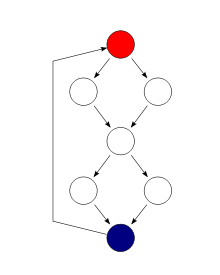
\includegraphics[width=0.5\textwidth]{../includes/pics/ciclomatica.png}
    \caption{Immagine complessità ciclomatica}
    \end{center}
\end{figure}
Tale indice può essere applicato a metodi, moduli e packages di un programma per limitare la complessità durante lo sviluppo. Durante la fase dei test è possibile utilizzare l'indice per determinare il numero di test necessari in quanto fornisce un limite superiore da non eccedere.
\begin{itemize}
    \item \textbf{Range accettazione}: [0 - 30];
    \item \textbf{Range ottimale}: [0 - 10].
\end{itemize}
\subsubsection{MPRDS010 - Numero di metodi}
Questa metrica calcola la media di occorrenze di metodi per ciascun package ed è utile poiché questi ultimi non dovrebbero contenere troppe definizioni di metodi. Un numero superiore alla media potrebbe indicare la necessità di una maggiore suddivisione del package in questione.
\begin{itemize}
    \item \textbf{Range di accettazione}: [2 - 10];
    \item \textbf{Range ottimale}: [3 - 8].
\end{itemize}
\subsubsection{MPRDS011 - Variabili non utilizzate}
Il linguaggio \markg{Java} consente la creazione di variabili che possono non essere mai effettivamente utilizzare e quindi inutili. Questo tipo di variabili verrà individuato utilizzando un tool apposito chiamato \textit{ProGuard}\footnote{\href{https://en.wikipedia.org/wiki/ProGuard\_{}software}{https://en.wikipedia.org/wiki/ProGuard\_{}software}} che si occuperà anche di questo compito, fra i tanti altri oneri di ottimizzazione che gli spettano.
Non vi è nessun range di accettazione o alcun range ottimale da definire in quanto il valore di questa metrica deve sempre essere pari a 0.

\subsubsection{MPRDS012 - Numero di bug per linea}
Questa metrica è utile per quantificare il numero di bug presenti su una certa regione di codice, composta da un certo numero di linee. Rendendo il codice più chiaro e semplice possibile si ridurrà la probabilità di introdurre bug: il rischio di introdurre bug aumenta con il crescere del numero di righe di codice.
\begin{itemize}
    \item \textbf{Range di accettazione}: [0 - 60];
    \item \textbf{Range ottimale}: [0 - 25].
\end{itemize}
\subsubsection{MPRDS013 - Rapporto linee di codice e commento}
Questa metrica riguarda le linee di codice prodotte in rapporto con le linee di commento, escludendo le righe vuote. L'indicazione principale riguarda la manutenibilità del codice. Un rapporto troppo basso indica una carenza di informazioni necessarie alla comprensione del codice.
\begin{itemize}
    \item \textbf{Valore accettabile}: rapporto \textgreater { 0.20};
    \item \textbf{Valore ottimale}: rapporto \textgreater { 0.30}.
\end{itemize}
\subsubsection{MPRDS014 - Code Coverage}
\label{sec:CodeCoverage}
Per poter avere una misura di codice verificato e testato si adotterà il Code Coverage che si calcola nel seguente modo:
\begin{center}
	\begin{displaymath}
	CC = \frac{NMT}{TNMT} * 100
	\end{displaymath}
\end{center}
Dove NMT indica il numero di metodi sottoposti a test mentre TNMT indica il numero di metodi da sottoporre a test.
Verrà utilizzato il tool JaCoCo\footnote{\href{https://www.jetbrains.com/help/idea/code-coverage.html}{https://www.jetbrains.com/help/idea/code-coverage.html}} che è integrabile all'interno dell'\markg{IDE} IntelliJ \markg{IDEA} e Android Studio per il linguaggio Java. Per quanto riguarda Node.js si farà affidamento a \footnote{\href{https://mochajs.org/}{https://mochajs.org/}}.

\subsection{Verifica}
\label{sec:verifica}
\subsubsection{Descrizione}
In questa sezione verranno descritti gli strumenti ed i metodi impiegati per la verifica del codice e dei documenti durante la loro realizzazione.
\subsubsection{Analisi statica}
L’analisi statica è una tecnica applicabile al codice ed alla documentazione che permette la verifica di un prodotto individuandone gli errori. Può essere svolta secondo:
\begin{itemize}
    \item \textbf{Inspection}: si applica quando si ha un’idea delle possibili problematiche che si stanno cercando e si effettua facendo una comparazione tra il prodotto e una tabella di possibili errori creata in precedenza;
    \item \textbf{Walkthrough}: si applica quando non si sa quali sono le tipologie di errori che si stanno cercando. Occorre ispezionare tutto il codice o il documento per trovare qualsiasi tipo di anomalia.
\end{itemize}
\subsubsection{Analisi dinamica}
L’analisi dinamica consiste nella creazione ed esecuzione di una serie di test direttamente sul codice, utilizzando anche dei tool già realizzati appositamente per tali scopi. Non è possibile fare analisi dinamica sui documenti.
\subsubsection{Verifica diagrammi UML}
I verificatori avranno il compito di controllare tutti i diagrammi UML ed assicurarsi che rispettino lo standard UML.

\subsection{Specifica dei test}
\label{sec:specifica_test}
\subsubsection{Scopo}
\label{sec:test_scopo}
Per garantire la qualità del prodotto e quindi la rilevazione degli errori durante la fase di sviluppo verrà fatta particolare attenzione sull'analisi dinamica del codice per mezzo di test automatici.
\subsubsection{Tipologia dei Test}
\label{sec:tipologia_test}
Sono state create tre macro categorie di test sulla base di tre tipologie di errore per la loro identificazione:
\begin{itemize}
	\item \textbf{Test di modulo} per verificare la logica del software;
	\item \textbf{Test ad alto livello} per verificare le funzionalità del sistema;
	\item \textbf{Test di regressione} per verificare i test precedenti dopo una modifica.
\end{itemize} 
\paragraph{Test di modulo}\mbox{}\\[0.4cm]
I test di questa tipologia si occupano della \markg{verifica} logica del software e verranno creati ed eseguiti dai programmatori. Il successo di questi test costituirà il vincolo per poter consegnare/caricare il codice all'interno della \markg{repository}.
Essi si dividono in:
\begin{itemize}
	\item \textbf{Test di unità - TU}\\
	Si verifica le parti di lavoro prodotte dal programmatore che corrispondo a piccole parti di codice e unità logiche, come ad esempio una classe, un metodo o funzione, oppure un insieme di essi.
	Si va quindi a isolare dal resto del codice una piccola parte di software testabile, chiamata \textit{unità}. Bisogna dunque stabilire se questa \textit{unità} funziona esattamente come previsto prima di poterla stabilmente integrare nella versione principale del software. L'approccio al test di unità verrà affidato ad un apposito framework di testing chiamato \footnote{\href{https://junit.org/junit5/}{JUnit}}.
	\item \textbf{Test di integrazione - TI}
	Si verifica l'integrazione tra le unità logiche che formano i vari componenti del sistema. Si verifica quindi che i componenti del sistema non contengano errori dovuti all'integrazione tra unità;
	Per testare l'integrazione si è scelto la tecnica dal basso verso l'alto, ovvero si testano per prime le parti con minore dipendenza funzionale e con maggiore funzionalità e successivamente risalire l'albero delle dipendenze.	
\end{itemize} 
\paragraph{Test ad alto livello}\mbox{}\\[0.4cm]
I test di questa tipologia si occupano di verificare le funzionalità del sistema, ovvero sul comportamento dell'applicazione, e gestire dai verificatori (team di \markg{Quality Assurance - QA}). Maggior parte di questi test sono manuali e per garantirne la loro organizzazione verrà gestita tramite degli apposti tool che verranno discussi in sede di Technology Baseline.
\begin{itemize}
	\item \textbf{Test funzionali - TF}\\
	Si verifica l'implementazione delle specifiche del prodotto concentrandosi sulle funzionalità delle suddette specifiche. Tali test sono visti come dei test di unità ad alto livello, difatti l'analisi della struttura è delegata ai Test di unità - TU.
	Questi test possono essere automatizzati e scritti dai programmatori, ma vengono affiancati ad una revisione ed esecuzione svolta dai verificatori;
	\item \textbf{Test di sistema - TS}\\
	Si verifica il sistema e l'architettura nella sua interezza. Il test di sistema sancisce quindi la validazione del software finale, giunto ad una release definitiva, e verifica che esso soddisfi tutti i requisiti in modo completo. Tali test sono complessi e pesanti, la loro implementazione verrà discussa in sede di Technology Baseline. Necessario l'utilizzo di componenti software supervisionati dai verificatori, quindi eseguiti dal team di \markg{Quality Assurance - QA};
	\item \textbf{Test di validazione - TV}\\
	Sono dei test finali che hanno il compito di valutare se il sistema sviluppato corrisponde alle richieste del proponente, quindi tali verifiche sono legate ai \markg{requisiti}. I test sono principalmente manuali ed eseguiti dal team \markg{Quality Assurance - QA}. Nelle fasi finali dello sviluppo verranno fatti i controlli assieme ai proponenti per determinale la validità del prodotto. 
\end{itemize} 
\paragraph{Test di regressione}\mbox{}\\[0.4cm]
I test di questa tipologia si occupa di rieseguire in modo selettivo i vari test, di modulo e di alto livello esclusi quelli di \markg{validazione}, elencati e descritti sopra. 
È quindi necessario l'esecuzione di questi test ogni qual volta che il codice viene modificato: l'inserimento di nuove funzionalità, la correzione di un bug o la modifica di parti del codice sorgente comporta l'esecuzione di tutti i test relativi ad essa. Vengono fatti questi test a fronte del fatto che l'introduzione di modifiche, migliorie e/o correzioni all'interno del codice è fortemente propenso all'inserimento di errori. I test di modulo necessari per la consegna nella \markg{repository} vengono eseguiti automaticamente, mentre per i test ad alto livello i verificatori pianificheranno l'esecuzione ad ogni superamento di \markg{baseline}.
\paragraph{Tracciamento dei test}\mbox{}\\[0.4cm]
Ogni test è strutturato nel seguente modo:
\begin{itemize}
	\item Codice identificativo
	\item Descrizione
	\item Stato
\end{itemize}
La sintassi scelta per il codice identificativo è la seguente:
\begin{center}
	\textbf{T\{tipo\}\{codice\}}
\end{center}
dove l'attributo \textbf{tipo} può essere:
\begin{itemize}
	\item \textbf{U}: Test di unità;
	\item \textbf{I}: Test di integrazione;
	\item \textbf{F}: Test funzionali;
	\item \textbf{S}: Test di sistema;
	\item \textbf{V}: Test di validazione;
\end{itemize}
mentre l'attributo \textbf{codice} è un numero incrementale che parte da 1 ed è associato al test di unità. Lo stato del test può essere uno dei seguenti:
\begin{itemize}
	\item Implementato;
	\item Non implementato;
	\item Superato;
	\item Non superato;
\end{itemize}


\subsubsection{Strumenti}
\begin{itemize}
    \item \textbf{Software}:  per la stesura del codice Java, si utilizzeranno gli IDE \emph{Intellij IDEA} e \emph{Android Studio}. Per la stesura del codice javascript per Node.js si utilizzerà \emph{Visual Studio Code};
    \item \textbf{Documenti}: per il controllo dei documenti verranno utilizzate le funzioni integrate a TexStudio per controllare che non ci siano errori nei file LaTeX. Verrà utilizzato GlossaryHelper per la gestione del glossario e per controllare che non vi siano presenti duplicati;
    \item \textbf{Gestione di processi e feedback}: verrà utilizzato il sistema di issues di GitLab;
    \item \textbf{Gestione di tasklist}: si utilizzeranno le funzionalità di Task Management di \markg{Asana}, un servizio cloud che crea dei \markg{task} ed assegna ad ogni membro un periodo temporale entro il quale svolgere il proprio operato;
    \item \textbf{Gestione del time tracking}: si utilizzeranno le funzionalità di Clockify (applicazione di time tracking free);
    \item \textbf{Analisi dinamica}: L'analisi dinamica sarà estesa a tutto il software prodotto e consiste in test di unità tramite libreria di testing \markg{JUnit};
    \item \textbf{Tracciamento dei requisti}: verrà utilizzato un tool chiamato \emph{ProgmaDB} per tracciare i requisti installando lo strumento su un \markg{server} remoto condiviso.
\end{itemize}
\subsection{Validazione}
\label{sec:validazione}
\subsubsection{Descrizione}
Il processo di \markg{validazione} ha come scopo quello della verifica del prodotto al fine di assicurarsi che sia conforme a quanto stabilito.
\subsubsection{Procedure}
L’attività di validazione verrà svolta secondo i seguenti passi:
\begin{enumerate} 
    \item \textbf{Tracciamento}: tracciamento dei test con report da parte dei verificatori.
    \item \textbf{Analisi dei risultati}: in seguito al punto 1, spetterà al Responsabile di progetto l’analisi dei report e la decisione di:
    \begin{itemize}
        \item Accettare la validazione e consegnare al proponente i risultati, informandolo sulle modalità di esecuzione della validazione;
        \item Ripetere i test in toto o in parte aggiungendo indicazioni mirate al miglioramento della fase di test che deve essere nuovamente eseguita.
    \end{itemize}
\end{enumerate}

